% Appendix: Cost Heuristic Validation

\section{Cost Heuristic Validation}
\label{sec:cost_heuristic_validation}

The selection utility (Equation~\ref{eq:budget_ucb}) uses a static log-normalized cost
$\tilde{c}_a$ derived from each model's blended per-token rate rather than the
realised per-request cost.  We validate this design choice by testing two
necessary conditions: (i)~$\tilde{c}_a$ preserves the \emph{true cost ranking}
across prompts, and (ii)~within-model cost variance is small relative to
inter-model gaps in log-cost space.

\paragraph{Blending assumption.}
The heuristic blends input and output pricing with equal weight
(i.e., a 1:1 token ratio).  In practice the output-to-input ratio varies
across models and prompts, so the blended rate differs from the true per-request
effective rate.  Because cost ranking depends only on the \emph{relative order}
of effective rates and the log-normalization compresses the dynamic range,
a simple average preserves the ranking whenever the price gap between models
exceeds the variation introduced by differing output lengths---a condition
satisfied for models spanning at least one order of magnitude in pricing.
Note that Llama-8B's blended rate (\$0.10/M tokens) coincides with the
market cost floor, so $\tilde{c}_{\text{Llama}} = 0$ by construction;
any model priced at or below the floor is treated as zero-cost in the
utility computation.

\paragraph{K=3 portfolio (\chNPromptsK{} shared val prompts; sanity check).}
The heuristic ordering Llama-8B $<$ Mistral-Large $<$ Gemini-Pro matches the
per-request cost ordering on \chFullOrderK\% of prompts
(95\,\% Wilson CI: [\chFullOrderKCILo, \chFullOrderKCIHi]\%).
All three pairwise comparisons hold at ${\geq}$\chMinPairwiseK\% under
strict inequality, with zero ties observed.
This result is unsurprising given the ${\sim}$500$\times$ cost span between
the cheapest and most expensive arm (per-model CVs in \chCVRangeK),
and serves primarily as a sanity check that the dataset is internally consistent.

\paragraph{K=4 portfolio (\chNPromptsKFour{} shared val prompts, with Gemini-Flash).}
Adding a fourth arm whose pricing overlaps an existing arm provides
a harder test of the heuristic.
For a clean comparison, we restrict both portfolios to the shared prompt subset:
\chKFourMissing{} prompts from the original K=3 validation split are excluded
because they are absent from the K=4 data file (excluded during Flash data
collection, likely due to API refusals or empty responses).
Gemini-Flash ($\tilde{c} = \chFlashCtilde$) is placed between Mistral-Large
($\tilde{c} = \chMistralCtilde$) and Gemini-Pro ($\tilde{c} = \chProCtilde$).
The full ordering matches on \chFullOrderKFour\%
(CI: [\chFullOrderKFourCILo, \chFullOrderKFourCIHi]\%) of prompts;
the closest pair (Mistral-Large vs.\ Gemini-Flash) preserves ranking on
\chMistralFlashPW\%
(CI: [\chMistralFlashPWCILo, \chMistralFlashPWCIHi]\%;
\chMistralFlashTies{} exact ties),
reflecting Flash's high cost variance (CV${} = \chFlashCV$) and the
narrow heuristic gap ($\Delta\tilde{c} = \chMistralFlashGap$).

\paragraph{Log-cost separation.}
To quantify tier separation without referencing the heuristic itself, we
examine per-model distributions in $\log(\text{cost}_{\text{USD}})$ space.
Within-model standard deviations are \chLogStdFracRange\% of the total
inter-model log-cost range, confirming that prompt-level cost noise does not
overwhelm tier separation.
Cohen's $d$ for adjacent pairs ranges from \chMinCohensD{}
(Mistral-Large $\to$ Gemini-Flash) to \chMaxCohensD{}
(Llama-8B $\to$ Mistral-Large); the weakest separation corresponds to the
only pair where the ranking inverts on ${\sim}$20\% of prompts.

\paragraph{Prompt-cost correlation.}
Spearman correlations between prompt word count and per-request cost are
statistically significant but modest in magnitude
($\rho = \chCorrRange$; all $p < 10^{-4}$).
The explained variance ($\rho^2 < 7\%$) suggests that prompt-level features
capture only a small fraction of cost variation, limiting the practical benefit
of a contextual cost model in this portfolio.

\paragraph{Cross-model cost correlation.}
Per-request costs are moderately to strongly correlated across models
($\rho = \chCrossCorrRange$), driven by shared output-length variation.
This shared factor preserves relative ordering even when absolute costs vary
widely (CV = \chCVRangeKFour).

\paragraph{Takeaway.}  The static $\tilde{c}_a$ heuristic is empirically
well-calibrated for portfolios where models span at least one order of
magnitude in pricing.  For denser price clusters (e.g., Mistral-Large
vs.\ Gemini-Flash, $d = \chMFCohensD$),
the ranking holds for ${\sim}$\chMistralFlashPW\% of prompts but inverts when
Flash generates unusually short responses.
Three structural properties limit downstream impact:
(i)~$\tilde{c}_a$ enters only the soft penalty
(Eq.~\ref{eq:budget_ucb}); the hard ceiling and the pacer's EMA cost
signal operate on actual per-request costs, so heuristic errors cannot
cause budget violations.
(ii)~For closely priced arms the absolute penalty gap is small
(${\sim}0.015$ for Mistral--Flash at $\lambda_t{=}0$)---negligible
relative to the $[0,1]$ reward signal.
(iii)~The dual variable $\lambda_t$ updates on actual costs
(Eq.~\ref{eq:dual_update}), self-correcting any persistent
over-selection of a costly arm.

\begin{figure}[!htbp]
\centering
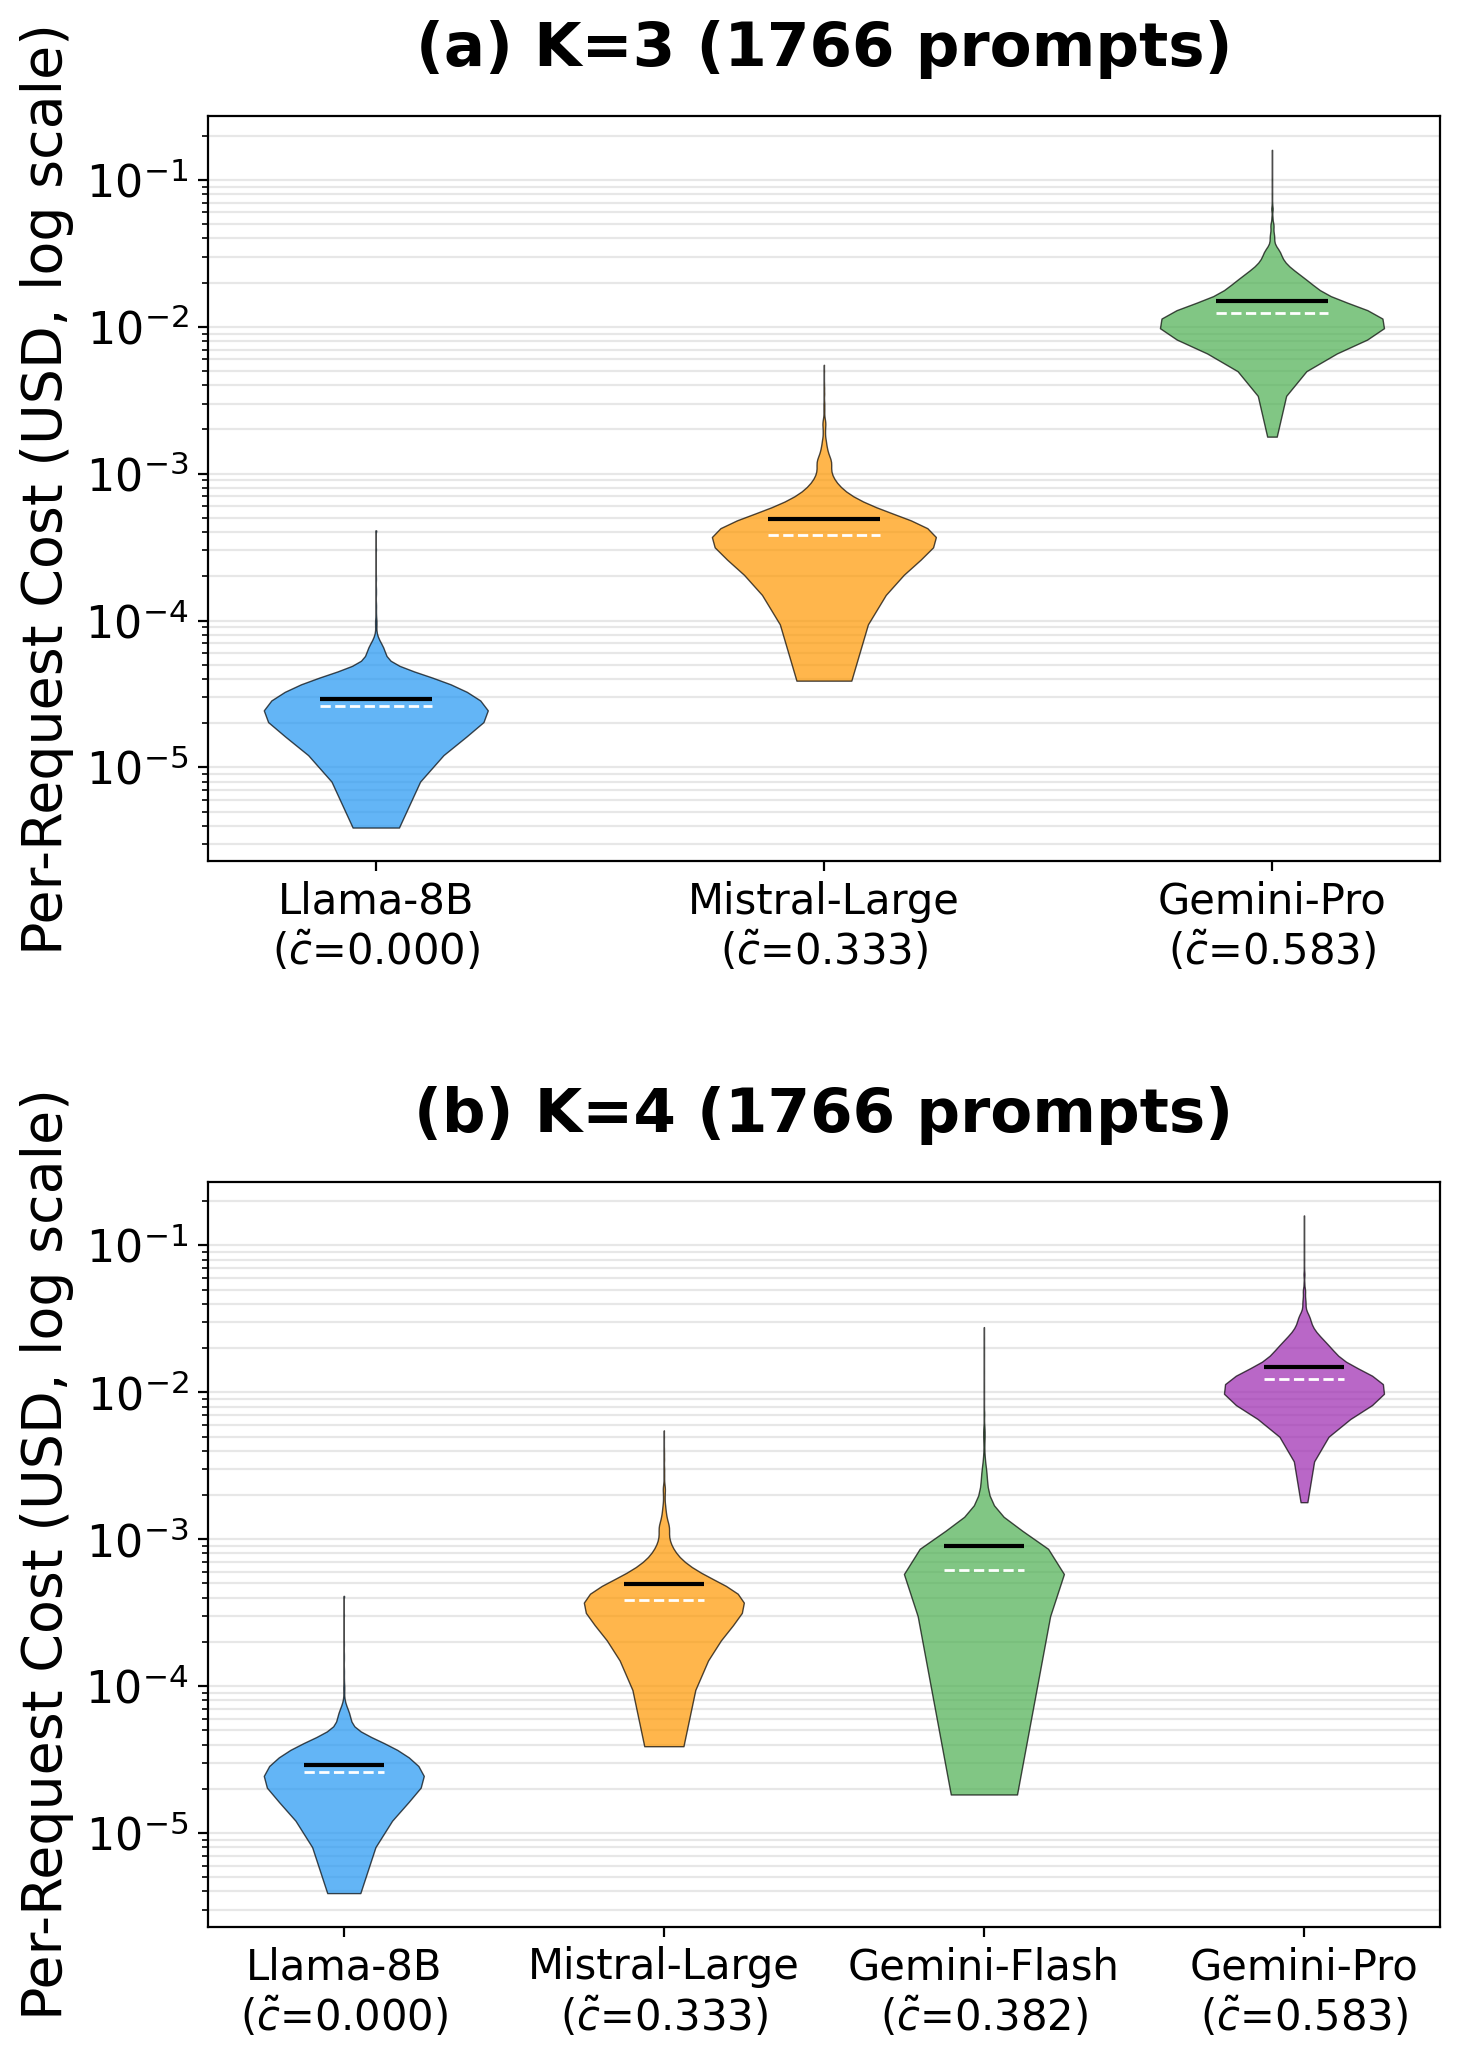
\includegraphics[width=\columnwidth]{../experiments/appendix/cost_heuristic_validation/results/cost_heuristic_validation_distributions.png}
\caption{Cost heuristic validation: realised cost distributions. Panel (a) shows per-request realised cost distributions for the $K{=}3$ portfolio on the shared validation subset, and panel (b) shows the same diagnostic for the $K{=}4$ portfolio. In both cases the violin plots are ordered by the static log-normalized heuristic $\tilde{c}_a$, illustrating that the major cost tiers are cleanly separated, with only the Mistral-Large and Gemini-Flash distributions showing substantial overlap.}
\label{fig:cost_heuristic_distributions}
\end{figure}

\begin{figure}[!htbp]
\centering
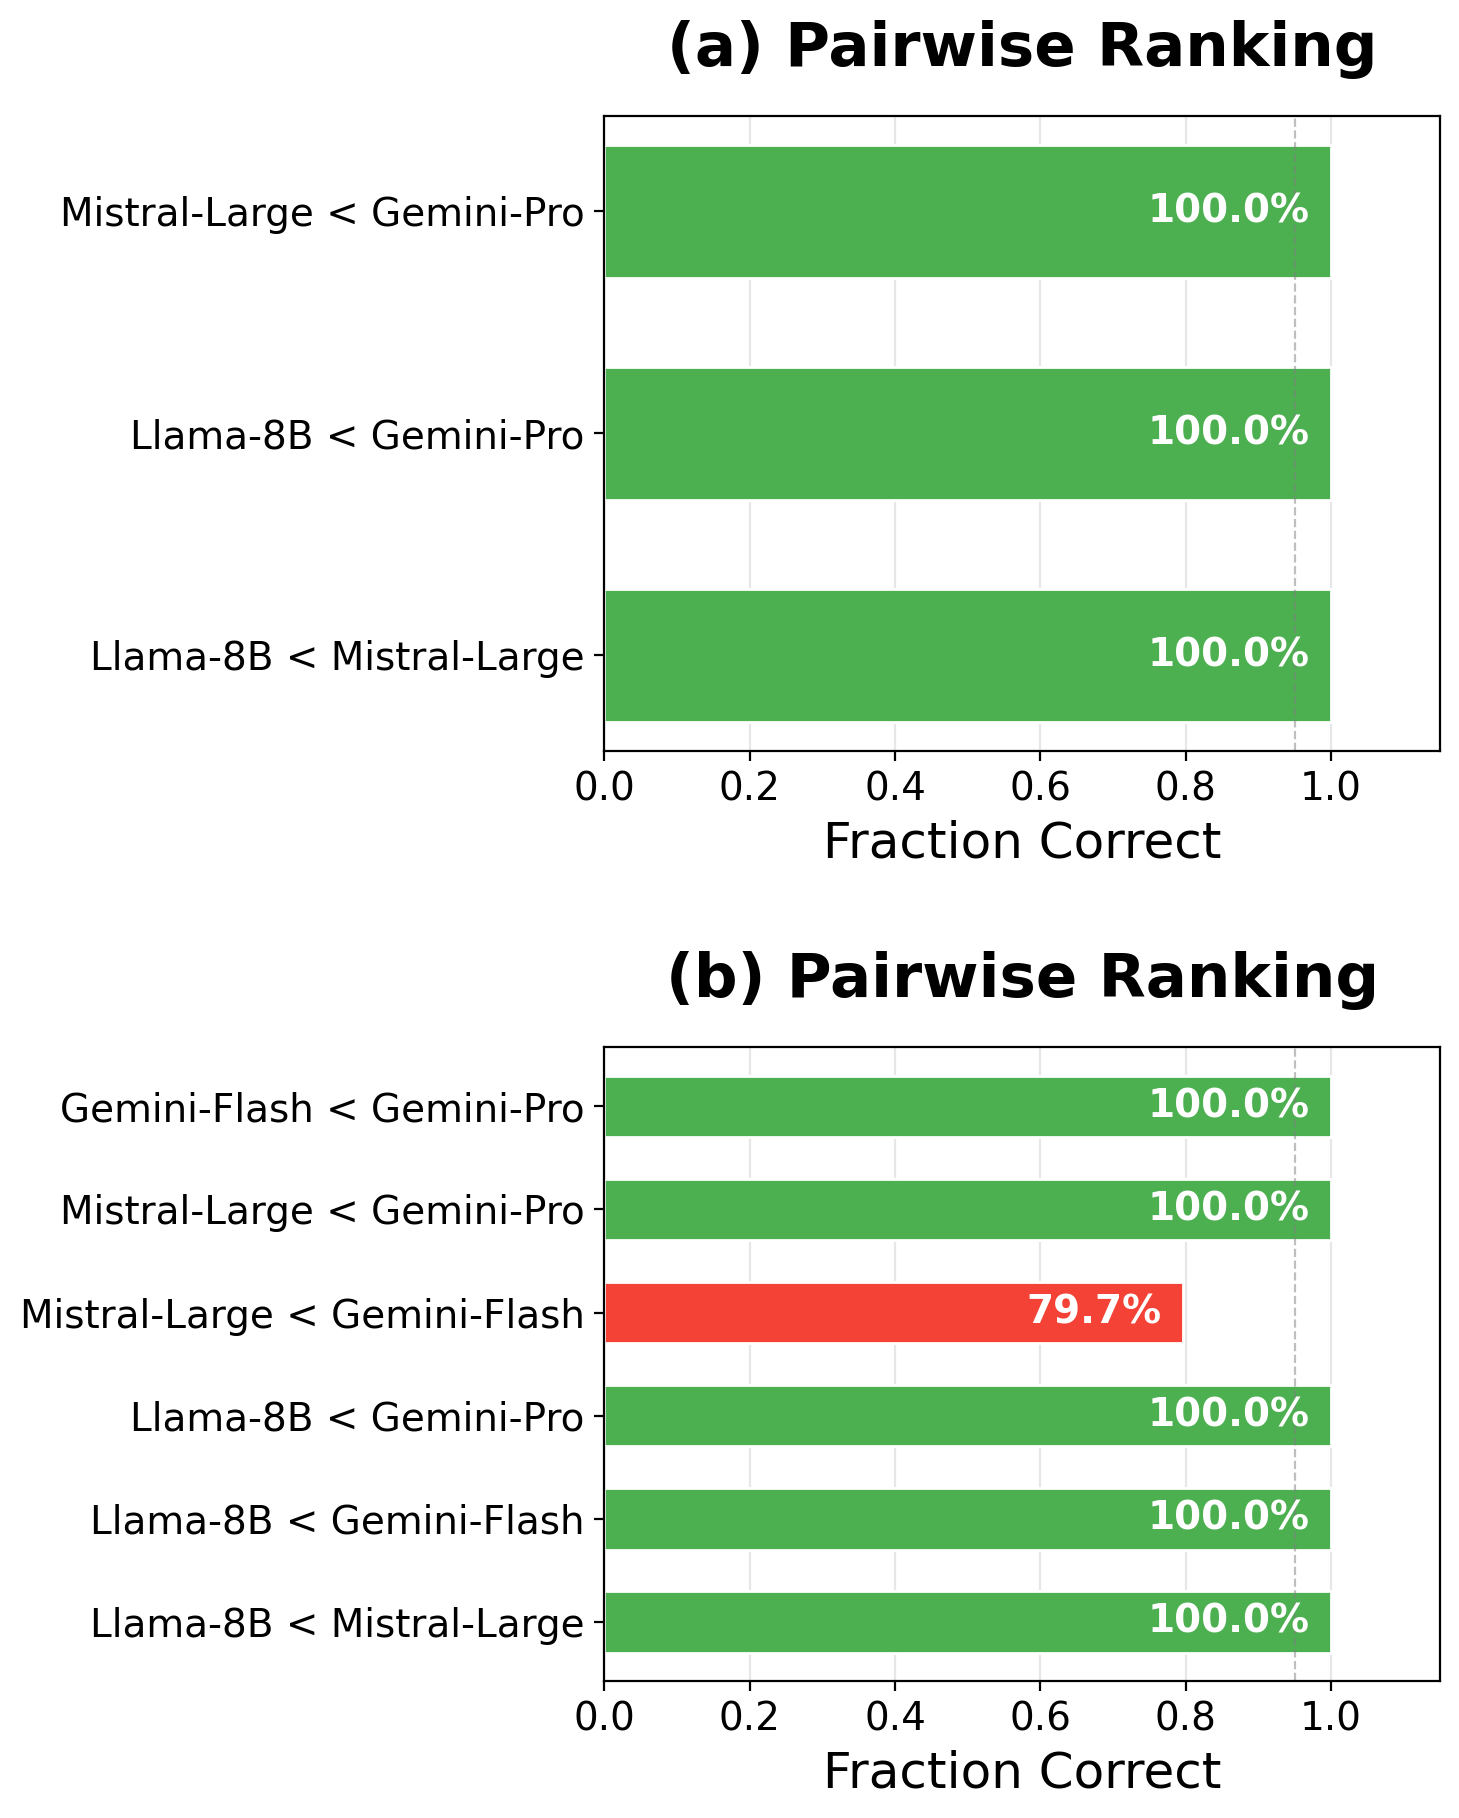
\includegraphics[width=\columnwidth]{../experiments/appendix/cost_heuristic_validation/results/cost_heuristic_validation_ranking.png}
\caption{Cost heuristic validation: ranking preservation. Subplot (a) shows pairwise ranking preservation for the $K{=}3$ portfolio on the shared validation subset, and subplot (b) shows the same diagnostic for the $K{=}4$ portfolio. The heuristic preserves the full per-request cost ordering on 100\% of shared-subset $K{=}3$ prompts and ${\sim}80\%$ of shared-subset $K{=}4$ prompts; the Mistral-Large vs.\ Gemini-Flash comparison is the only source of inversions.}
\label{fig:cost_heuristic_ranking}
\end{figure}
